 \documentclass[t]{beamer}
%\documentclass{beamer}
\listfiles

\mode<presentation>
{
  %\usetheme[deutsch,titlepage0]{KIT}
\usetheme[deutsch]{KIT}
% \usetheme{KIT}

%%  \usefonttheme{structurebold}

  \setbeamercovered{transparent}

  %\setbeamertemplate{enumerate items}[circle]
  \setbeamertemplate{enumerate items}[ball]

}
\usepackage{babel}
%\date{10.05.2010}
%\DateText

\newlength{\Ku}
\setlength{\Ku}{1.43375pt}

\usepackage[utf8]{inputenc}
\usepackage[TS1,T1]{fontenc}
\usepackage{array}
\usepackage{multicol}
\usepackage{lipsum}

%\usenavigationsymbols
%\usenavigationsymbols[sfHhdb]
%\usenavigationsymbols[sfhHb]

\title[]{Implementierung Croggle}
\subtitle{Praxis der Softwareentwicklung WS 13/14}
\author[]{Vincent Schüßler}

\AuthorTitleSep{\relax}

\institute[IPD]{Lukas Böhm \(\cdot\) Tobias Hornberger \(\cdot\) Jonas Mehlhaus \(\cdot\) Iris Mehrbrodt  \(\cdot\) Vincent Schüßler \(\cdot\) Lena Winter}

\TitleImage[width=\titleimagewd]{images/title}

\newlength{\tmplen}

\newcommand{\verysmall}{\fontsize{6pt}{8.6pt}\selectfont}

\begin{document}

\begin{frame}
  \maketitle
\end{frame}

\begin{frame}
	
\includegraphics[width=\textwidth]{images/screenshots/menu}
\end{frame}

\begin{frame}[c]
	\begin{center}
	\Huge
	Musskriterien
	\end{center}
\end{frame}

\begin{frame}
	\frametitle{Bearbeiten \& Auswerten}
	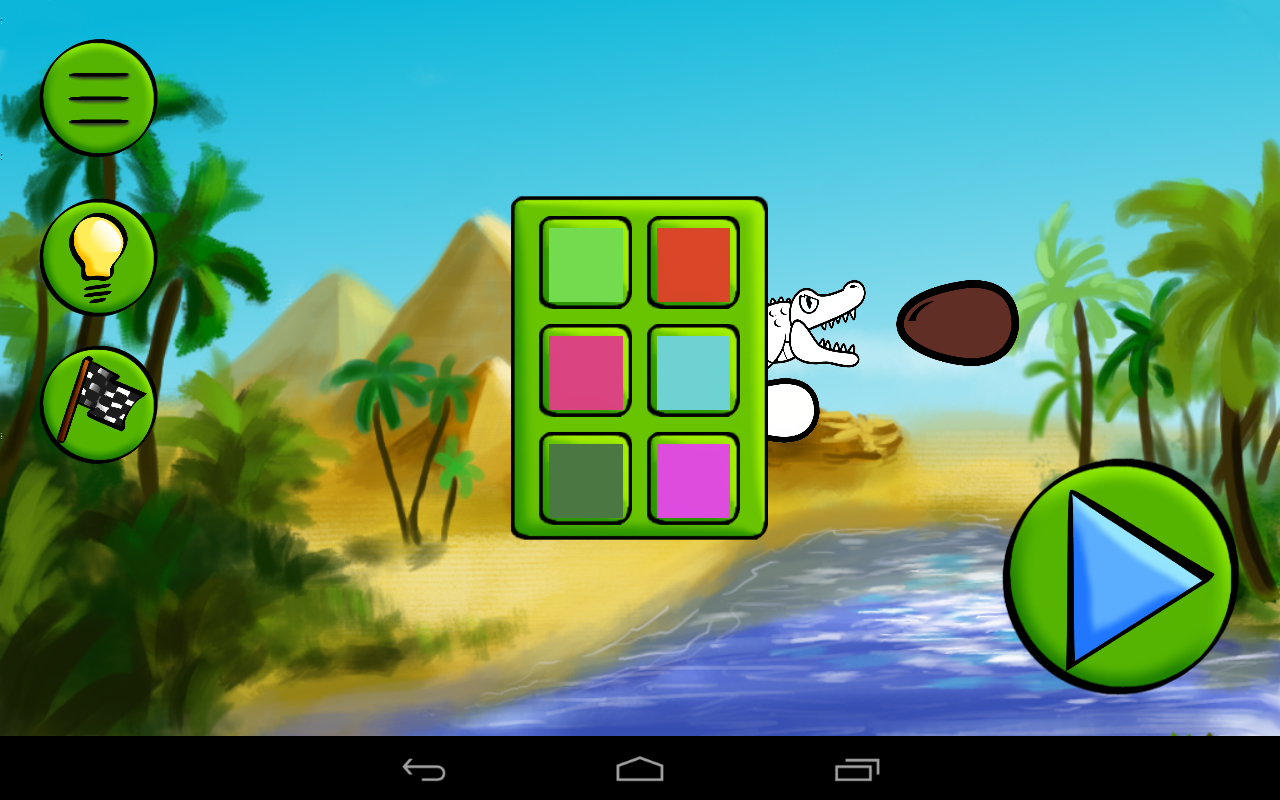
\includegraphics[width=\textwidth]{images/screenshots/color_edit}
\end{frame}

\begin{frame}
	\frametitle{Bearbeiten \& Auswerten}
	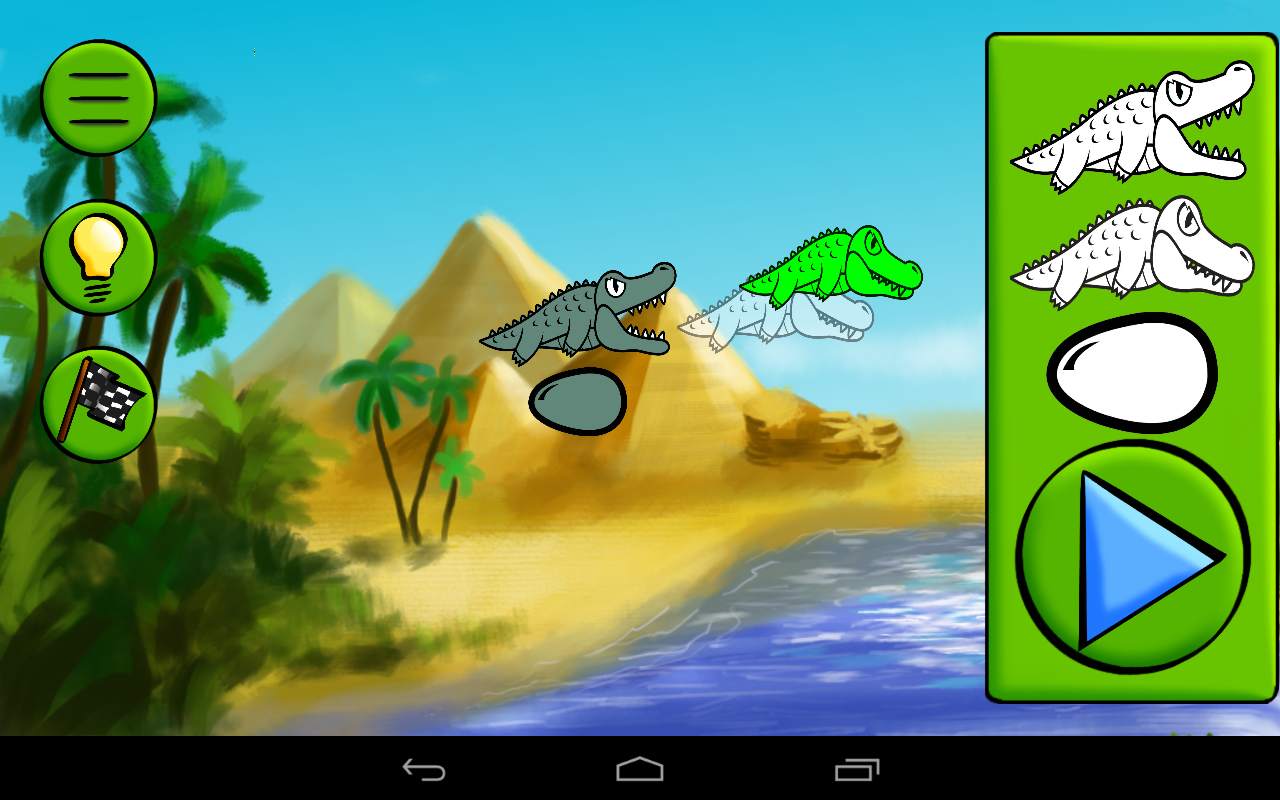
\includegraphics[width=\textwidth]{images/screenshots/term_edit}
\end{frame}

\begin{frame}
	\frametitle{Bearbeiten \& Auswerten}
	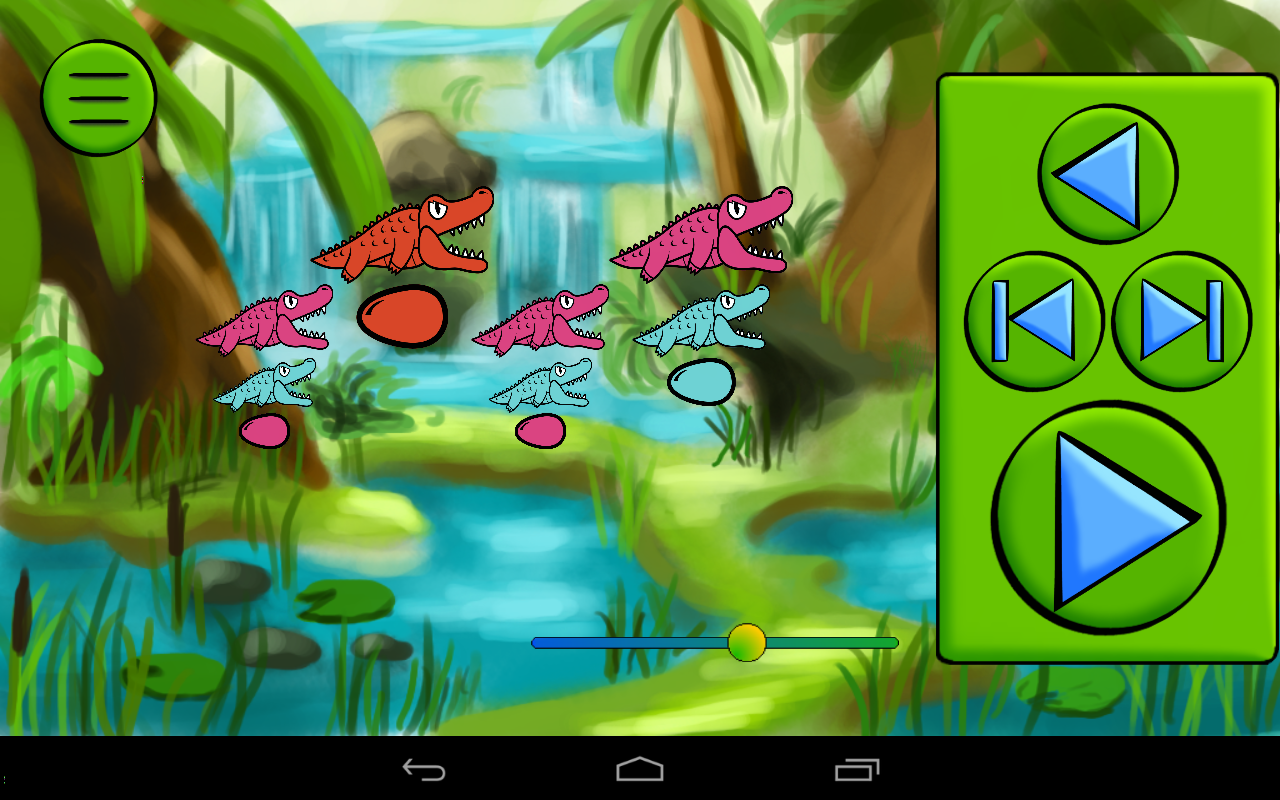
\includegraphics[width=\textwidth]{images/screenshots/simulation}
\end{frame}

\begin{frame}
	\frametitle{Lernfortschritt}
	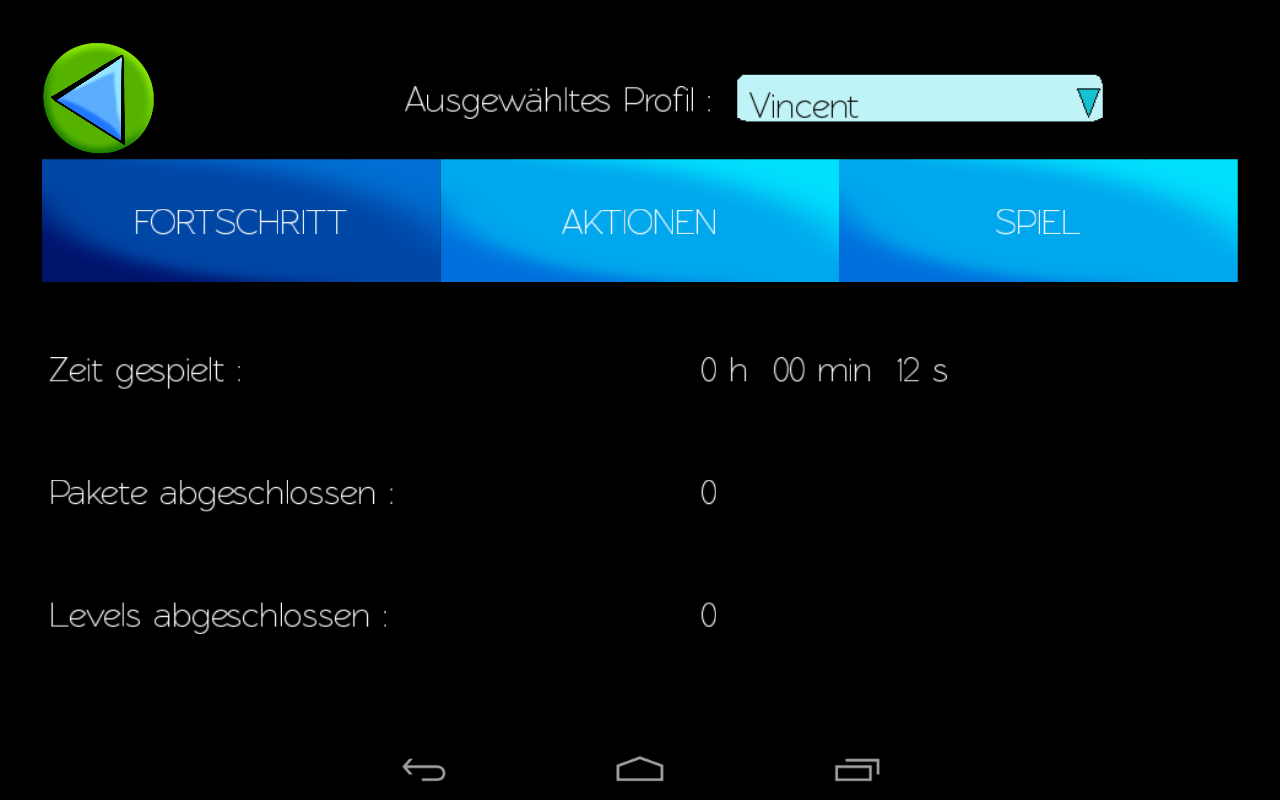
\includegraphics[width=\textwidth]{images/screenshots/progress}
\end{frame}

\begin{frame}
	\frametitle{Interaktive Einführung}
	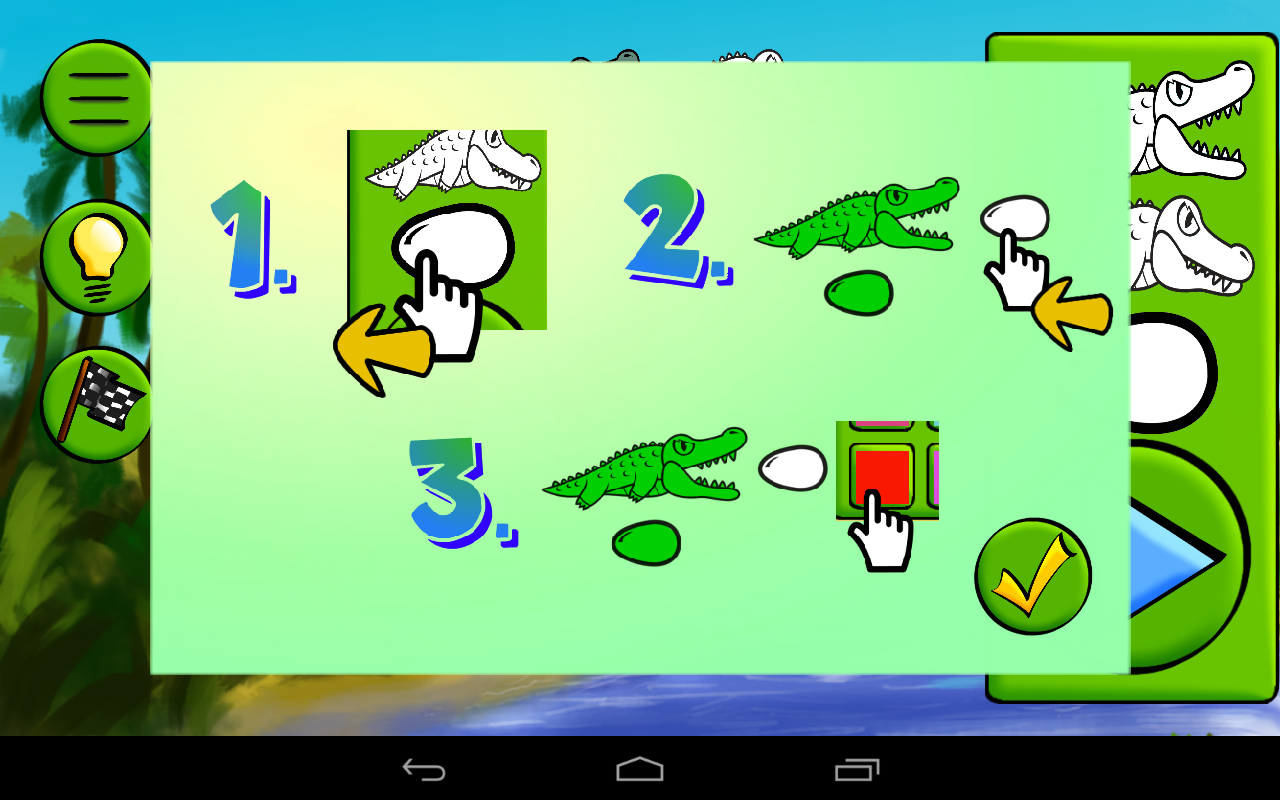
\includegraphics[width=\textwidth]{images/screenshots/tutorial}
\end{frame}

\begin{frame}
	\frametitle{Langzeitmotivation}
	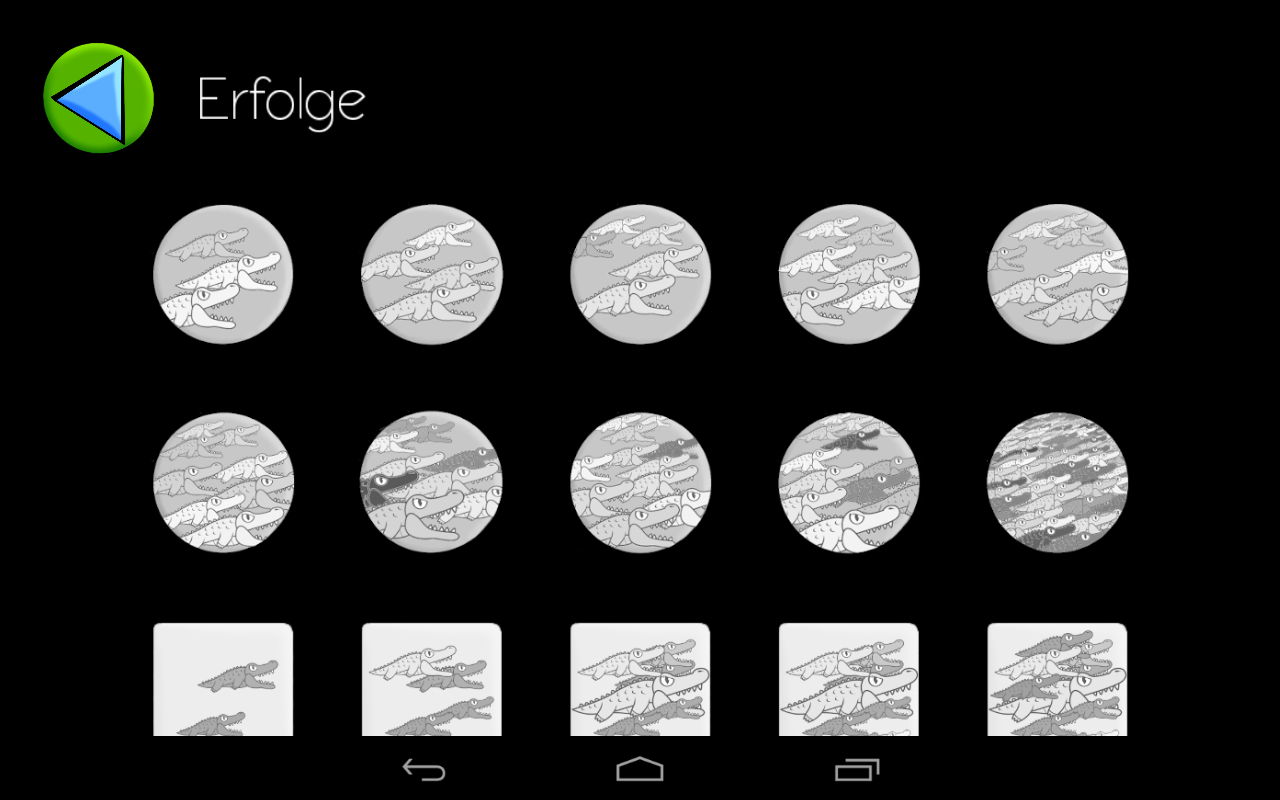
\includegraphics[width=\textwidth]{images/screenshots/achievements}
\end{frame}

\begin{frame}[c]
	\begin{center}
	\Huge
	Umgesetzte Wunschkriterien
	\end{center}
\end{frame}

\begin{frame}
	\frametitle{Mehrere Benutzer}
	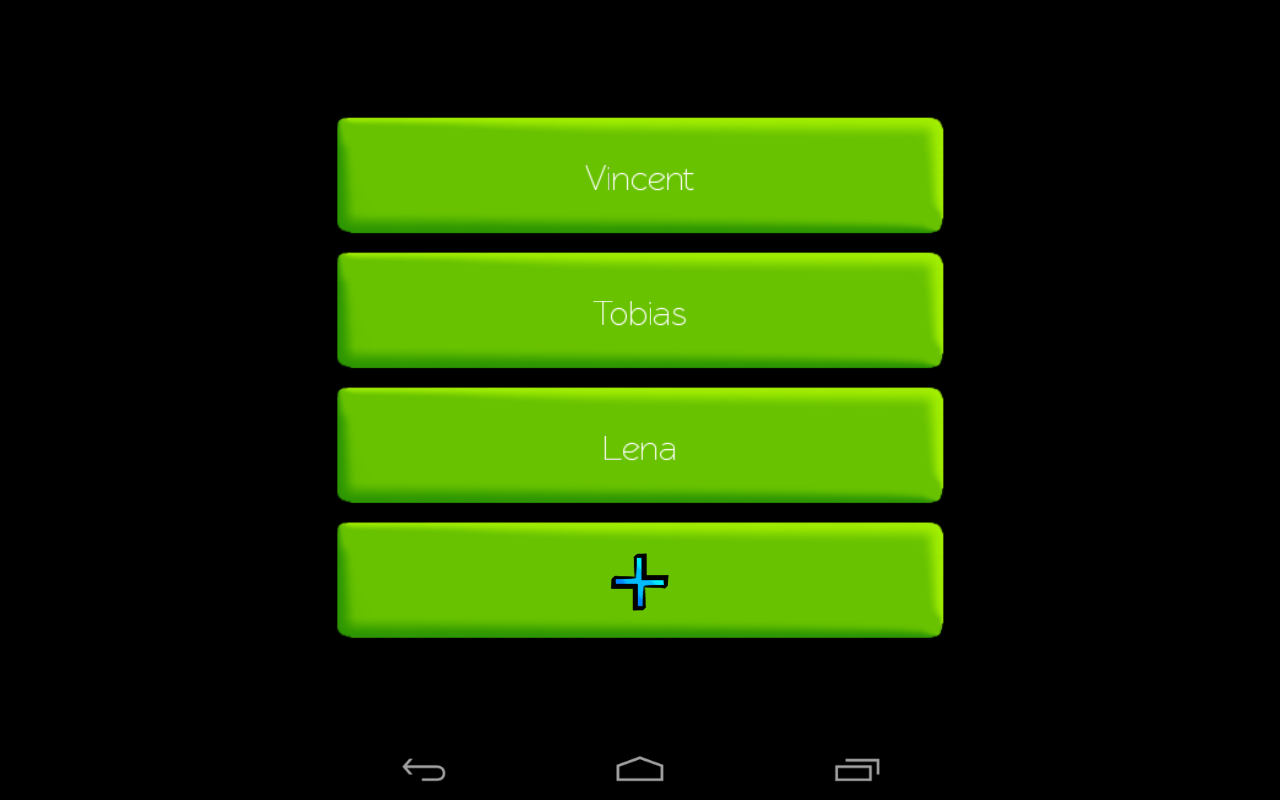
\includegraphics[width=\textwidth]{images/screenshots/users}
\end{frame}

\begin{frame}
	\frametitle{Verschiedene Leveltypen}
	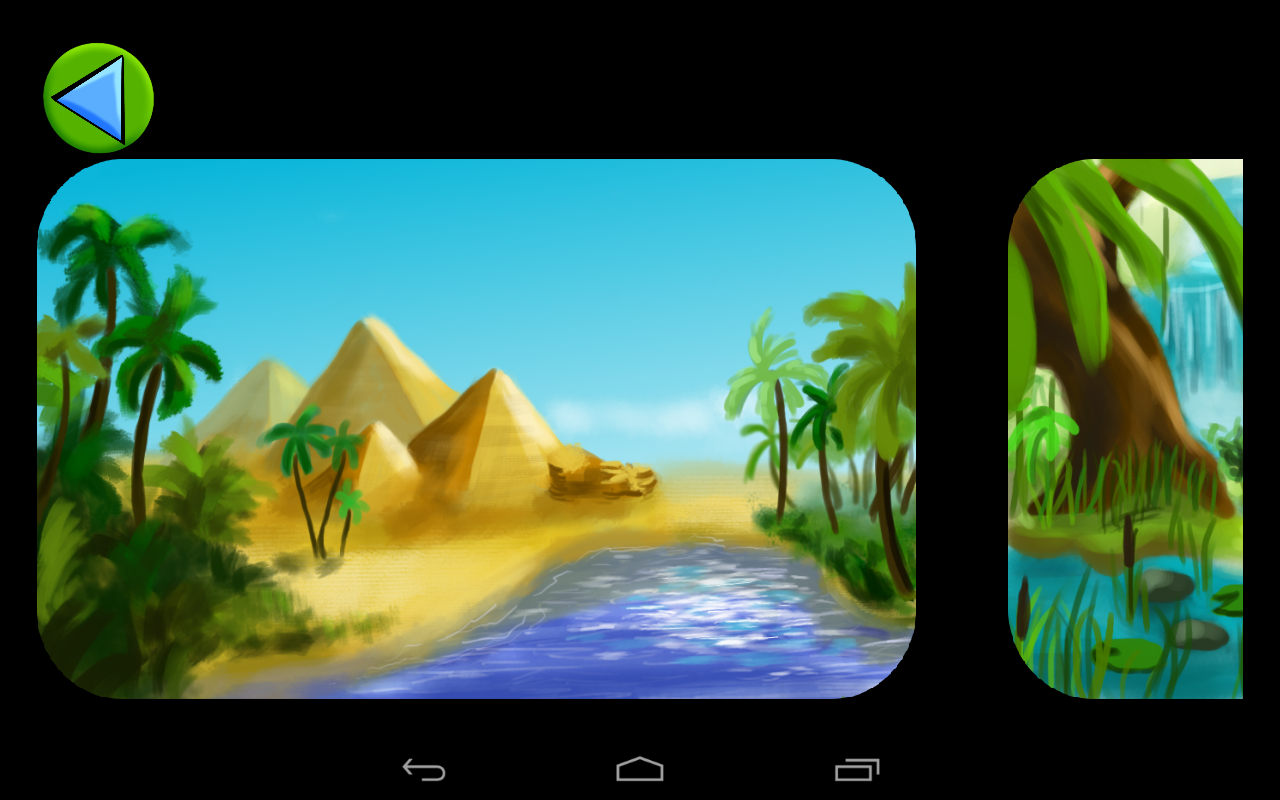
\includegraphics[width=\textwidth]{images/screenshots/packages}
\end{frame}

\begin{frame}
	\frametitle{Verschiedene Leveltypen}
	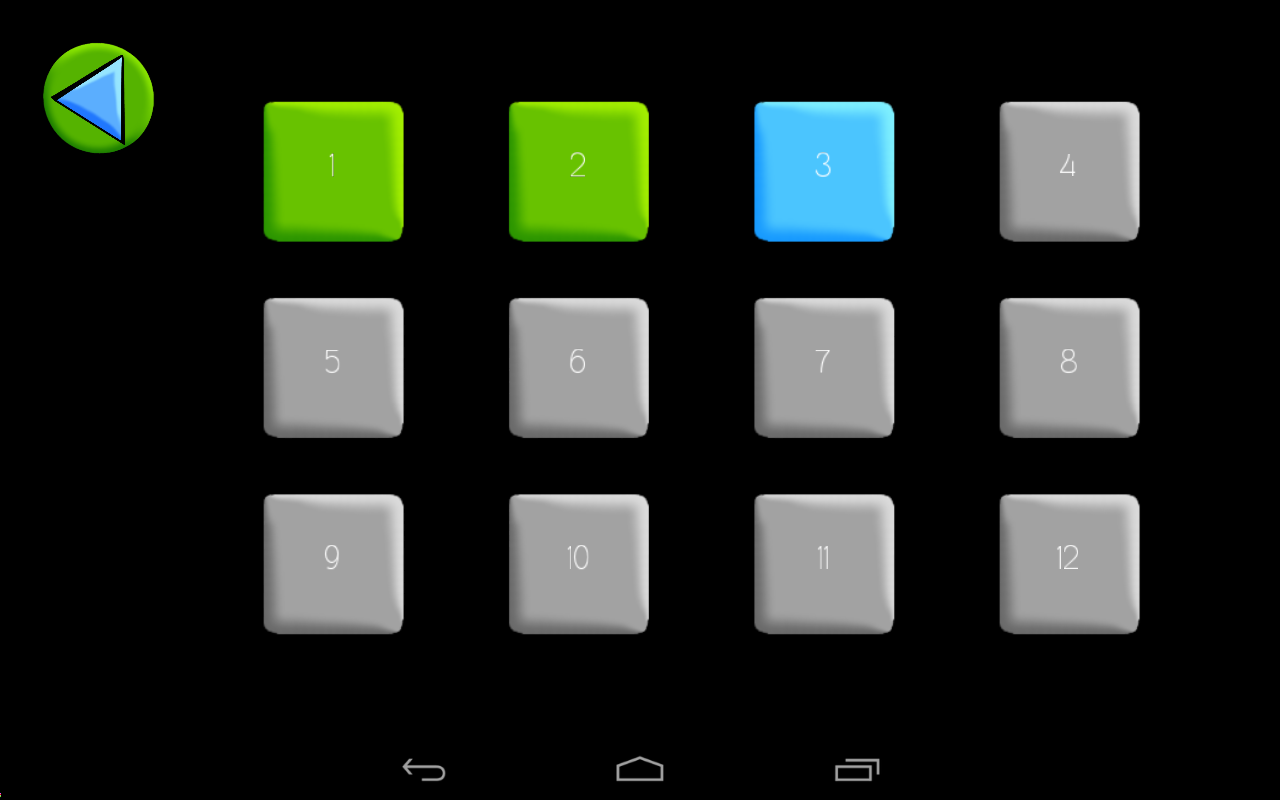
\includegraphics[width=\textwidth]{images/screenshots/levels}
\end{frame}

\begin{frame}
	\frametitle{Verschiedene Leveltypen}
	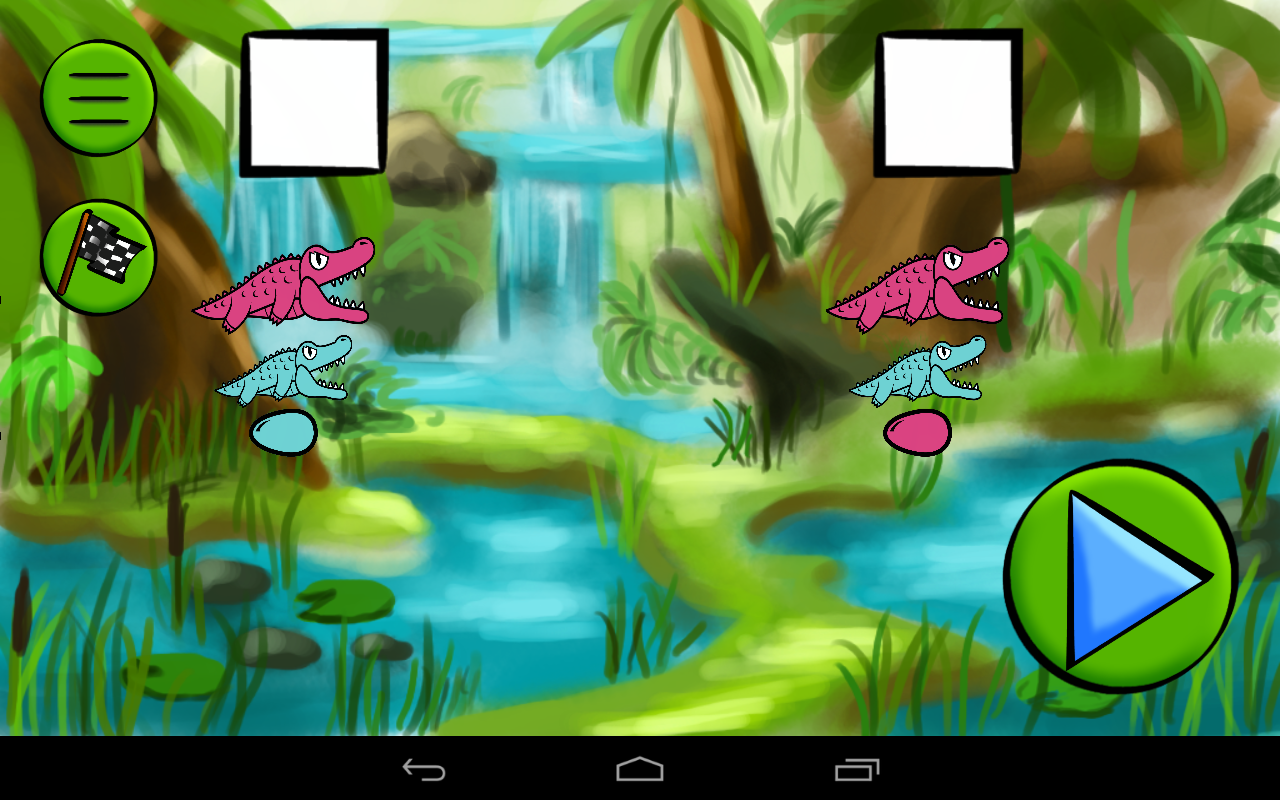
\includegraphics[width=\textwidth]{images/screenshots/multiple_choice}
\end{frame}

\begin{frame}
	\frametitle{Farbenblindenmodus}
	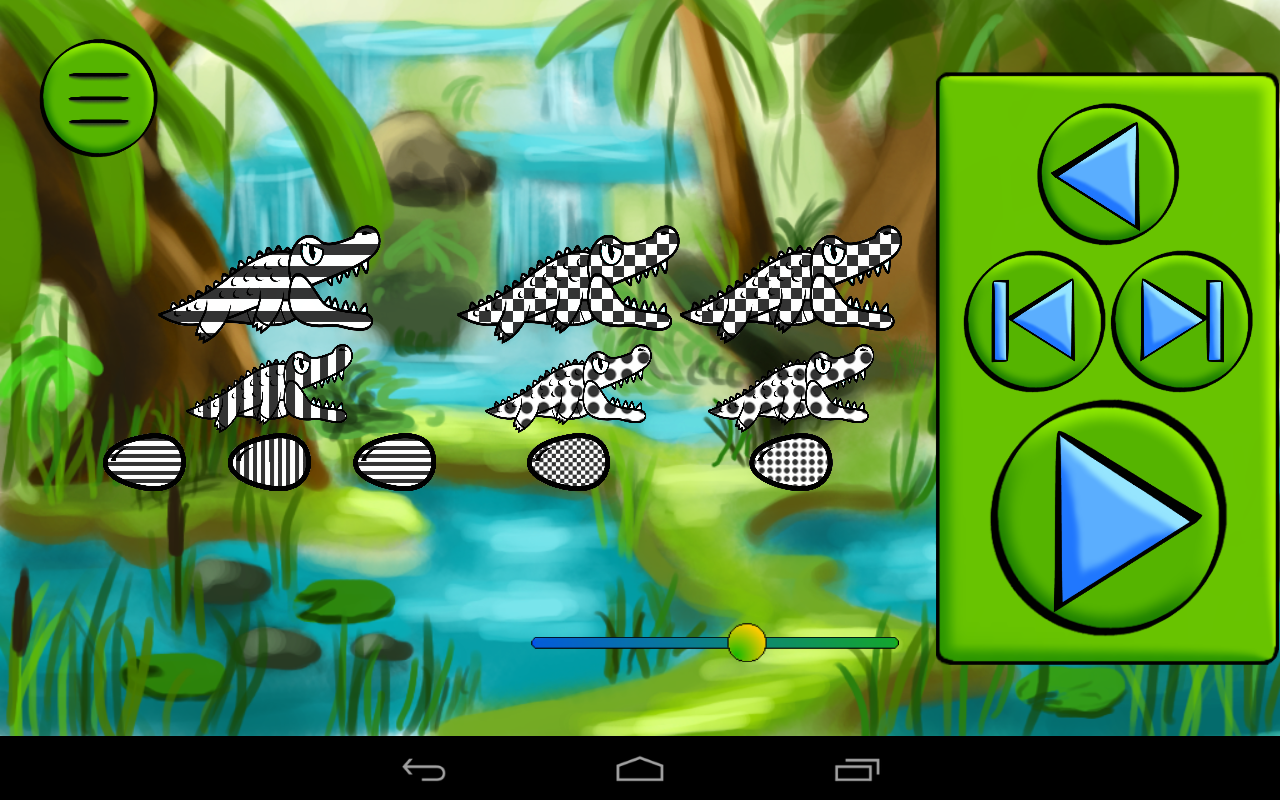
\includegraphics[width=\textwidth]{images/screenshots/colorblind}
\end{frame}

\begin{frame}[c]
	\frametitle{Gestrichene Wunschkriterien}
	\begin{itemize}
		\item Angepasste Version für Smartphones
		\item Vermittlung einer Geschichte durch Animationen
	\end{itemize}
\end{frame}

\end{document}
